\documentclass[tikz,border=10pt]{standalone}
\usepackage{tikz}
\usetikzlibrary{calc}

\begin{document}
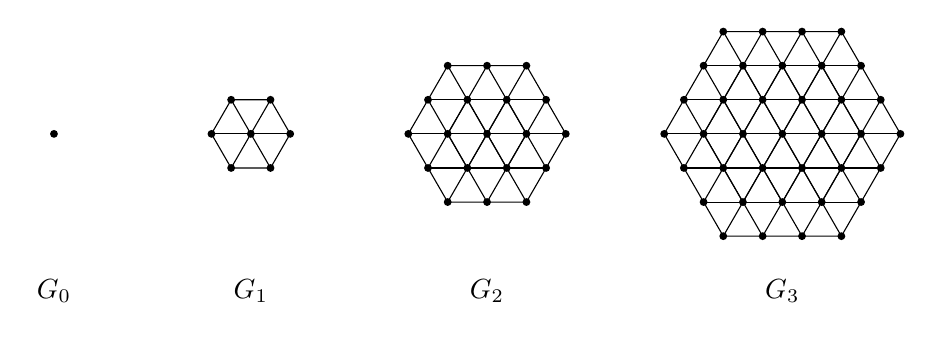
\begin{tikzpicture}[dot/.style={circle, fill=black, inner sep=1pt}]

%─────────────
% Controls
%─────────────
\def\hexstep{0.5}  % Distance from center to first ring point (controls scale)
\definecolor{olivegreen}{rgb}{0.33,0.42,0.18}  % Custom olive green

%─────────────────────────────────────────────────────────────
% Draws a hexagonal lattice of dots:
%─────────────────────────────────────────────────────────────
\newcommand{\drawHexagonDots}[3]{%
  \begin{scope}[shift={({#2},{#3})}]

    \pgfmathtruncatemacro{\rings}{#1}

    \ifnum\rings<1
      \node[dot] at (0,0) {};
    \else
      % Draw the central dot
      \node[dot] at (0,0) {};

      % Special case: draw edges from the center if rings ≥ 1
      \foreach \a in {0,60,...,300} {
        \draw[thin] (0,0) -- ++(\a:\hexstep);
      }

      % Loop over each ring
      \foreach \r in {1,...,\rings} {
        \pgfmathsetmacro{\rad}{\r * \hexstep}

        % Each ring is a hexagon with 6 sides
        \foreach \side in {0,...,5} {
          \pgfmathsetmacro{\angleA}{60*\side}
          \pgfmathsetmacro{\angleB}{60*(\side+1)}

          \coordinate (A) at (\angleA:\rad);
          \coordinate (B) at (\angleB:\rad);

          % Place dots evenly along each edge
          \foreach \k in {0,...,\numexpr\r-1} {
            \pgfmathsetmacro{\t}{\k/\r}
            \coordinate (P) at ($(A)!{\t}!(B)$);
            \node[dot] at (P) {};

            % Only draw spokes for non-outer rings
            \ifnum\r<\rings
              \foreach \a in {0,60,...,300} {
                \draw[thin] (P) -- ++(\a:\hexstep);
              }
            \fi
          }
        }
      }
    \fi

    % Draw hexagon outline around the outer ring
    \pgfmathsetmacro{\outerrad}{\rings * \hexstep}
    \path (0:\outerrad) coordinate (P0);
    \path (60:\outerrad) coordinate (P1);
    \path (120:\outerrad) coordinate (P2);
    \path (180:\outerrad) coordinate (P3);
    \path (240:\outerrad) coordinate (P4);
    \path (300:\outerrad) coordinate (P5);
    \draw[thin] (P0) -- (P1) -- (P2) -- (P3) -- (P4) -- (P5) -- cycle;

  \end{scope}
}

%─────────────
% Manually draw in selected nodes
%─────────────
\newcommand{\selectPoint}[2]{%
  \node[circle, draw=olivegreen, fill=white] at ({#1},{#2}) {}; 
  \node[dot, fill=olivegreen] at ({#1},{#2}) {}; 
}
 
% H_0 through H_3
%─────────────
% Draw examples H₁ through H₃
%─────────────
\drawHexagonDots{0}{-4.5}{0}     % H0 = 1
\drawHexagonDots{1}{-2}{0}     % H₁ = 7
\drawHexagonDots{2}{1}{0}     % H₂ = 19
\drawHexagonDots{3}{ 4.75}{0}  % H₃ = 37

 

%─────────────
% Labels
%─────────────
\node at (-4.5,-2) {$G_0$};
\node at (-2,-2) {$G_1$};
\node at ( 1,-2) {$G_2$};
\node at ( 4.75,-2) {$G_3$};
\end{tikzpicture}
\end{document}